% !TEX root = ./paper.tex

\subsection{Performance Variations on Different Training Datasets}\label{sec:justify}

We constructed a benchmark suite with the programs from the DaCapo suite,
and used 3$\sim$4 small programs (i.e. luindex, lusearch, antlr, and pmd$_{m}$) as our training set.
In this subsection, we evaluate \ourtool~on different combinations of training data to see how its performance is affected by the number of training programs.

%Despite the small number and small size, they provide sufficient information to learn cost-effective heuristics,
%and we conducted an additional experiment to justify this evaluation setting.


We found that the amount of training data is overall critical, and
using four small programs as a training set can produce competitive heap abstraction heuristics cost-effectively.
Table~\ref{tbl:training} presents the performance and scores
(i.e. ${\mbox{\#proven casts}}\over{\mbox{analysis time (s)}}$)
of each heuristic learned with various combinations of training programs (i.e., \onepgm, \twopgm, \threepgm, and \fourpgm) and an ideal heuristic (\ideal) against the validation program findbugs.
For the ideal heuristic (\ideal), we assume that it has the precision of \Mahjong~and the scalability of \TypeBased~
since they are the most precise and the most scalable respectively in our space of heap abstraction heuristic.
The second row, analysis time (s), in table~\ref{tbl:training} indicates the amount of time each heuristic took to successfully analyze the validation program, and
the third row, \#proven casts, presents the number of castings proved to be safe;
thereby, the more precise the analysis, the greater the number of proven casts.
As shown in Table~\ref{tbl:training}, the score increases with respect to the size of training set.
The score of \fourpgm~(i.e. 13.6) is nearly the same with that of the ideal heuristic (i.e. 15.4) in our evaluation.
It implies that using four programs as a training set is sufficient to produce cost-effective heap abstraction heuristics.


% among the various combinations of our training programs.
%In Table~\ref{tbl:training}, \onepgm, \twopgm, \threepgm, and \fourpgm correspond to the heuristics learned with
%{\it npgm} $(1 \le n\le 4)$ indicates the number of training programs used for learning heuristics.
%We calculate the cost of the ideal heuristic with the cost of \TypeBased~and the proven queries by \Mahjong~
%because \TypeBased~is most scalable
%and \Mahjong~is most precise in our space of heap abstraction heuristics.
%
%
%The row score present the quality of the learned heuristics and an ideal heuristic
%
%The black solid line and red dotted line in the graph present the scores of our learned heuristics and an ideal heuristic (i.e.,
%${\small {\mbox{proven queries in \Mahjong}}\over{
%\mbox{cost of \TypeBased}}}$),
%respectively.
%We calculate the cost of the ideal heuristic with the cost of \TypeBased~and the proven queries by \Mahjong~
%because \TypeBased~is most scalable
%and \Mahjong~is most precise in our space of heap abstraction heuristics.
%\minseok{revision}

%In our experiments, we used 3 $\sim$ 4 programs for our training set.

%\textcolor{red}{
%Although we used a small number of small programs (e.g., luindex, lusearch, antlr, pmd$_{m}$) as a training set, those training programs do not represent unrealistic training data.

Using four programs as training programs could produce cost-effective heuristics because, even though our training programs are the smallest among the total benchmark programs,
they still provide sufficient learning data for our approach.
First, the DaCapo suite itself is a collection of realistic programs.
DaCapo has been carefully designed to include various behaviors and complex codes~\cite{Blackburn2006}.
For example, even the smallest program (i.e. lusearch) in Dacapo has more methods than the largest one in the SPEC benchmark~\cite{specjvm98}.
Secondly, when training heuristics in our approach, what matters is the number of allocation-sites, not the number of programs;
the learning algorithm of \OurCtx~treats individual allocation-sites as labelled data.
Our training programs provide sufficient training data to learn cost-effective heuristics in this sense.
%The training programs we used provide sufficient number of learning data.
More precisely, the smallest program (lusearch) has 4,752 allocation-sites,
and the remaining three training programs (lusearch, antlr, pmd$_{m}$) provide 14,068 unique allocation-sites in total;
we have a total of 18,820 allocation-sites for training data.
%}

%\textcolor{red}{
In practice, we recommend a user to choose programs with less than 400 classes as training programs, for which we found Grahpick typically works well. Although limited, our experience shows that a collection of such programs can provide useful training data.
%}
%\begin{table}[]
%\small
%\caption{Performance comparison among heuristics learned with various numbers (1$\sim$4) of training programs.}
%\label{tbl:training_pgms}
%\begin{tabular}{@{}clrrrr@{}}
%\toprule
%         & \multicolumn{1}{c}{} & \multicolumn{1}{c}{\onepgm} & \multicolumn{1}{c}{\twopgm} & \multicolumn{1}{c}{\threepgm} & \multicolumn{1}{c}{\fourpgm} \\ \midrule
%% \multirow{2}{*}{luindex}  & analysis time (s)    & 26(+27)                   & 41(+26)                   & 23(+50)                   & 23(+90)                   \\
%% %\multirow{2}{*}{luindex}  & analysis time (s)    & 26                   & 41                   & 23                   & 23                   \\
%%          & \#may-fail casts     & 358                       & 358                       & 358                       & 358                       \\ \bottomrule
%%\multirow{2}{*}{findbugs} & analysis time (s)    & 4,090               & 411                 & 153                 & 96                  \\
%\multirow{2}{*}{findbugs} & analysis time (s)    & 4,090(+185)               & 411(+107)                 & 153(+226)                 & 96(+363)                  \\
%         & \#may-fail casts     & 2,417                     & 1,768                      & 1,800                     & 1,774                     \\ \bottomrule
%\end{tabular}
%\end{table}
%
%
%\begin{figure}
%	\centering
%		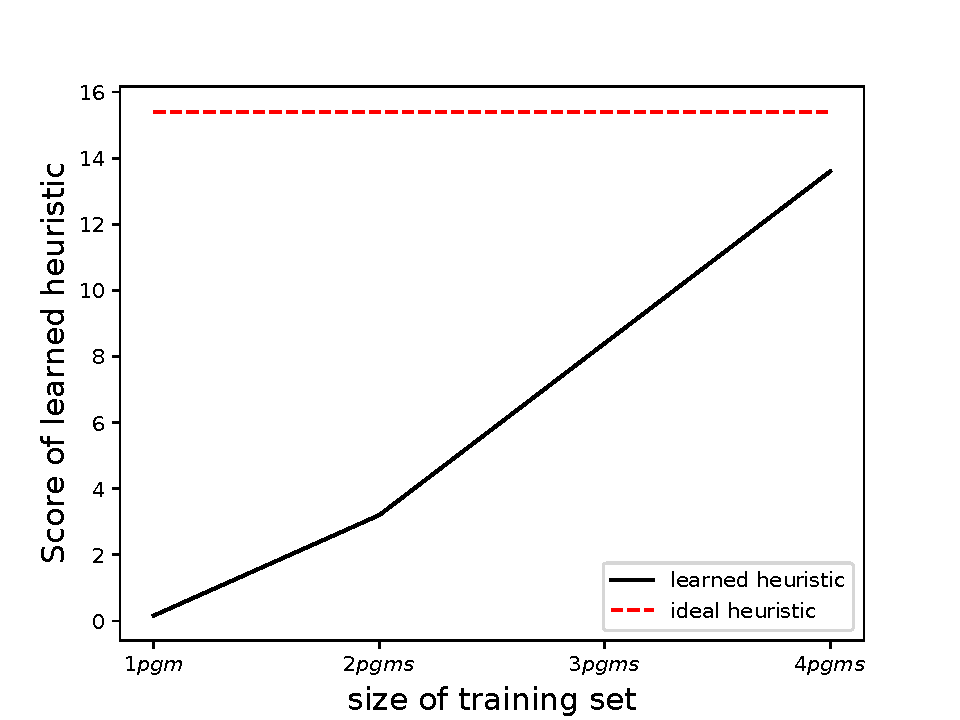
\includegraphics[width=7cm]{figures/training_set.pdf}
%	\caption{How score of learned heuristic changes over the value
%		of $\hyper$.}
%	\label{fig:training}
%\end{figure}


% Please add the following required packages to your document preamble:
% \usepackage{booktabs}
\begin{table}[]
\setlength\extrarowheight{-1pt}
\caption{Performance comparison among heuristics learned from various combinations of training sets (i.e. \onepgm, \twopgm, \threepgm, and \fourpgm) and an ideal heuristic (\ideal) against the validation program findbugs. \#proven casts presents the number of casts proved to be safe; a more precise analysis produces a larger number of \#proven casts.
The row score presents the quality of the heuristics computed by
${\mbox{\#proven casts}}\over{\mbox{analysis time (s)}}$.}
\label{tbl:training}
%${\projproved(F_P(\heuristic(G)))}\over{\projcost(F_P(\heuristic(G)))}$.}
\centering\scriptsize
\begin{tabular}{@{}lrrrrr@{}}
\toprule
%\multicolumn{1}{c}{} & \multicolumn{1}{c}{\onepgm} & \multicolumn{1}{c}{\twopgm} & \multicolumn{1}{c}{\threepgm} & \multicolumn{1}{c}{\fourpgm} & \multicolumn{1}{c}{\multirow{3}{*}{\ideal}} \\
\multicolumn{1}{c}{\multirow{2}{*}{}} & \multirow{2}{*}{\{luindex\}} & \multicolumn{1}{c}{\multirow{2}{*}{\{luindex, lusearch\}}} & \multicolumn{1}{c}{\{luindex, lusearch} & \multicolumn{1}{c}{\{luindex, lusearch} & \multicolumn{1}{c}{\multirow{2}{*}{\qquad\ideal}} \\
\multicolumn{1}{c}{} &  &  & \multicolumn{1}{c}{antlr\}}  & \multicolumn{1}{c}{antlr, pmd\}} &  \\ \midrule
analysis time (s)    & 4,090(+185)                                & 411(+107)                                  & 153(+226)                                    & 96(+363)                                    & 92                        \\
\#proven casts     & 672                                      & 1,321                                      & 1,289                                        & 1,315                                       & 1418                      \\ \midrule
score                & 0.16                   & 3.2                    & 8.4                      & 13.6                    & 15.4 \\\bottomrule
\end{tabular}
\end{table}


%\begin{figure}
%\vspace{-22pt}
%\begin{multicols}{2}
%~\\~\\~\\
%\begin{subfigure}[]{0.9\columnwidth}
%\small
%%\begin{tabular}{@{}c|lrr@{}}
%%\toprule
%%\multicolumn{1}{c}{}                          & \multicolumn{1}{c}{} & \multicolumn{1}{c}{\onepgm}   & \multicolumn{1}{c}{\twopgm}  \\ \midrule
%%\multirow{5}{*}{findbugs} & analysis time (s)    & 4,090(+185)                  & 411(+107)                   \\
%%                          & \#may-fail casts     & 2,417                        & 1,768                       \\ \cmidrule(){2-4}
%% & \multicolumn{1}{c}{} & \multicolumn{1}{c}{\threepgm} & \multicolumn{1}{c}{\fourpgm} \\
%%						  \cmidrule(){2-4}
%%                          & analysis time (s)    & 153(+226)                    & 96(+363)                    \\
%%                          & \#may-fail casts     & 1,800                        & 1,774                      \\\bottomrule
%%\end{tabular}
%\end{subfigure}
%
%\columnbreak
%\vspace{-57pt}
%\begin{subfigure}[t]{0.9\columnwidth}
%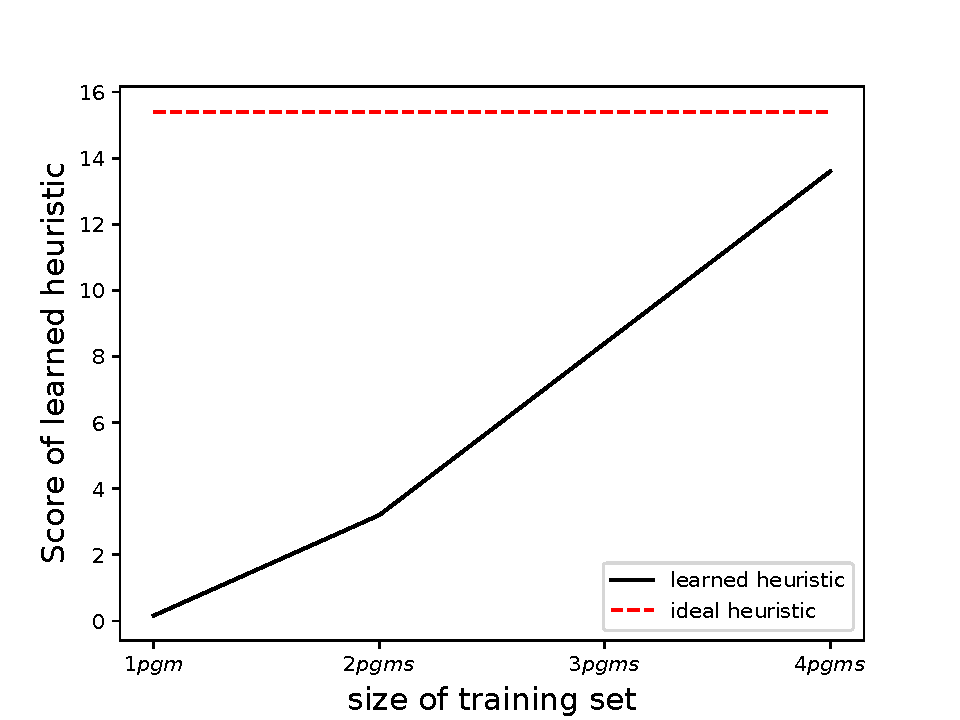
\includegraphics[width=7cm]{figures/training_set.pdf}
%\end{subfigure}
%\end{multicols}
%\vspace{-0.5cm}
%\caption{Performance of heuristics learned with various numbers (1$\sim$4) of training programs, and how score of learned heuristic changes over the size of training set.}
%\label{fig:training}
%\end{figure}

%
%	\centering
%	\begin{tabular}{cc}
%		% Please add the following required packages to your document preamble:
%% \usepackage{booktabs}
%% \usepackage{multirow}
%
%&
%		
%	\end{tabular}
%		of $\hyper$.}
%	\label{fig:gamma}
%






%%% Local Variables:
%%% mode: latex
%%% TeX-master: "paper"
%%% End: 